

\documentclass[notes=show,smaller]{beamer}
%%%%%%%%%%%%%%%%%%%%%%%%%%%%%%%%%%%%%%%%%%%%%%%%%%%%%%%%%%%%%%%%%%%%%%%%%%%%%%%%%%%%%%%%%%%%%%%%%%%%%%%%%%%%%%%%%%%%%%%%%%%%%%%%%%%%%%%%%%%%%%%%%%%%%%%%%%%%%%%%%%%%%%%%%%%%%%%%%%%%%%%%%%%%%%%%%%%%%%%%%%%%%%%%%%%%%%%%%%%%%%%%%%%%%%%%%%%%%%%%%%%%%%%%%%%%
\usepackage{amsmath}
\usepackage{mathpazo}
\usepackage{hyperref}
\usepackage{multimedia}

\setcounter{MaxMatrixCols}{10}

\newenvironment{stepenumerate}{\begin{enumerate}[<+->]}{\end{enumerate}}
\newenvironment{stepitemize}{\begin{itemize}[<+->]}{\end{itemize} }
\newenvironment{stepenumeratewithalert}{\begin{enumerate}[<+-| alert@+>]}{\end{enumerate}}
\newenvironment{stepitemizewithalert}{\begin{itemize}[<+-| alert@+>]}{\end{itemize} }
\usetheme{CambridgeUS}
\input{tcilatex}

\newcommand{\spcol}[1]{{\color{blue}{#1}}}
%\newcommand{\tcol}[1]{{\color{blue}{#1}}}
\newcommand{\bcol}[1]{{\color{blue}{#1}}}
\newcommand{\gcol}[1]{{\color{blue}{#1}}}
\newcommand{\nmcol}[1]{{\color{black}{#1}}}
\newcommand{\warning}[1]{{\color{blue}{#1}}}


\renewcommand{\Pr}{\mbox{P}}
\newcommand{\E}{\mbox{E}}
\newcommand{\se}{\mbox{se}}
\newcommand{\sres}{\widetilde{e}}
\newcommand{\Var}{\mbox{Var}}
\newcommand{\Cov}{\mbox{Cov}}
\newcommand{\Corr}{\mbox{Corr}}
\newcommand{\xbar}{\overline{x}}
\newcommand{\ybar}{\overline{y}}
\newcommand{\yhat}{\widehat{y}}

\newcommand{\Xbar}{\overline{X}}
\newcommand{\Ybar}{\overline{Y}}
\newcommand{\sx}{s_{\scriptscriptstyle x}}
\newcommand{\sX}{s_{\scriptscriptstyle X}}
\newcommand{\sy}{s_{\scriptscriptstyle y}}
\newcommand{\phat}{\hat{p}}
\newcommand{\phatX}{\hat{p}_{\scriptscriptstyle X}}
\newcommand{\that}{\hat{\theta}}

\newcommand{\mtbwin}[1]{\mbox{\sf [ #1 ]}}
\newcommand{\mtbwincom}[2]{\mbox{\sf [ #1 ]}\newline
{\sf [} #2 {\sf ]}}

\newenvironment{myverbatim}{
\renewcommand{\baselinestretch}{.85}\footnotesize\begin{alltt}}
{\renewcommand{\baselinestretch}{1}\end{alltt}}

\newcommand{\iid}{\stackrel{\mathrm{iid}}{\sim}}
\newcommand{\dd}{\stackrel{\mathrm{D}}{\sim}}

\newcommand{\Emis}{ {\bf E}^{{\rm mis}} }
\newcommand{\Umis}{ {\bf U}^{{\rm mis}} }
\newcommand{\bi}{\begin{itemize}}
\newcommand{\ei}{\end{itemize}}
\newcommand{\be}{\begin{equation}}
\newcommand{\ee}{\end{equation}}
\newcommand{\ba}{\begin{eqnarray}}
\newcommand{\ea}{\end{eqnarray}}
\newcommand{\ban}{\begin{eqnarray*}}
\newcommand{\ean}{\end{eqnarray*}}
\newcommand{\sig}{\sigma}
\newcommand{\mr}[1]{\mathrm{#1}}
\newcommand{\ep}{\varepsilon}
\newcommand{\bX}{\mbox{\boldmath{$X$}}}
\newcommand{\balpha}{\mbox{\boldmath{$\alpha$}}}
\newcommand{\bbeta}{\mbox{\boldmath{$\beta$}}}
\newcommand{\bTheta}{\mbox{\boldmath{$\Theta$}}}
\newcommand{\btheta}{\mbox{\boldmath{$\theta$}}}
\newcommand{\bsigma}{\mbox{\boldmath{$\sigma^2$}}}
\newcommand{\bgamma}{\mbox{\boldmath{$\gamma$}}}
\newcommand{\bmu}{\mbox{\boldmath{$\mu$}}}
\newcommand{\bldeta}{\mbox{\boldmath{$\eta$}}}
\newcommand{\bdelta}{\mbox{\boldmath{$\delta$}}}
\newcommand{\et}{{\it et al.}}
\newcommand{\bGamma}{\mbox{\boldmath{$\Gamma$}}}
\newcommand{\bLambda}{\mbox{\boldmath{$\Lambda$}}}
\newcommand{\N}{\mathcal{N}}



\newcommand{\logit}{\mbox{logit}}
\newcommand{\probit}{\mbox{probit}}
\newcommand{\hiw}{\mbox{HIW}}
%\newcommand{\N}{\mbox{N}}
\newcommand{\U}{\mbox{Unif}}
\newcommand{\C}{\mbox{C}}
%\newcommand{\Be}{\mbox{Be}}
%\newcommand{\dd}{\mbox{d}}
\newcommand{\IG}{\mbox{IG}}
%\newcommand{\Ga}{\mbox{Ga}}
%\newcommand{\Po}{\mbox{Po}}
\newcommand{\DP}{\mbox{DP}}
\newcommand{\AR}{\mbox{AR}}
\newcommand{\GP}{\mbox{GP}}
\newcommand{\DE}{\mbox{DE}}
%\newcommand{\Ex}{\mbox{Ex}}
%\newcommand{\E}{\mbox{E}}
%\newcommand{\Var}{\mbox{Var}}
\newcommand{\lp}{\mathit{l}^{\alpha}}
\newcommand{\IB}{\mbox{IB}}
\newcommand{\Z}{\mbox{Z}}
\newcommand{\GZ}{\mbox{GZ}}
\newcommand{\Meix}{\mbox{Meix}}
\newcommand{\Be}{\mbox{Be}}
\newcommand{\Ga}{\mbox{Ga}}

\newcommand{\bw}{\mathbf{w}}
\newcommand{\Xt}{X^{(t)}}
\newcommand{\psit}{\psi^{(t)}}
\newcommand{\psiT}{\psi^{(T)}}
\newcommand{\Zt}{Z^{(T)}}
\newcommand{\Sigmat}{\widehat{\Sigma}^{(t)}}
\newcommand{\phit}{\phi^{(t)}}
\newcommand{\omegat}{\omega^{(t)}}

\newcommand{\by}{\mathbf{y}}
\newcommand{\p}{p}


\def\sko {\vspace{.1in}}
\def\skoo {\vspace{.2in}}
\def\skooo {\vspace{.3in}}

\title[Quasi-convex SDP]{Quasi-convex Stochastic Dynamic Programming}
%\subtitle{Exponential Slice Sampler}
\author{John R. Birge}
\institute[Chicago Booth]{Chicago Booth}
\date[07/15]{ISMP Pittsburgh, July 2015}

\begin{document}
\begin{frame}
\maketitle
\end{frame}

%%%%%%%%%%%%%%%%%%%%%%%%%%%%%%%%%%%%%%%%%%%%%%%%%%%%%
\begin{frame}
\frametitle{Overview}

\footnotesize
Agenda

\begin{itemize}
\item Motivation from commodity storage management

\item Basic set-up: sample the corresponding Gibbs distribution
$$
\pi_\kappa (x) = \exp \left \{ - \kappa f(x) \right \} / Z_\kappa \; \; {\rm for} \; \; x \in \mathcal{X} \;
$$
where $ \kappa \in \{ 0 < \kappa_1 < \ldots < \kappa_m \} $: Simulated Tempering.

\item Wide variety of functional behaviour
\begin{enumerate}
\item Himmelblau, Rastigrin, Rosenbrock, Shubert
\end{enumerate}

\item Exponential Slice Sampler:  Swendsen-Wang Algorithm.
\end{itemize}



\end{frame}
%%%%%%%%%%%%%%%%%%%%%%
\begin{frame}

\begin{figure}[hbp]
%\vspace{-1in}
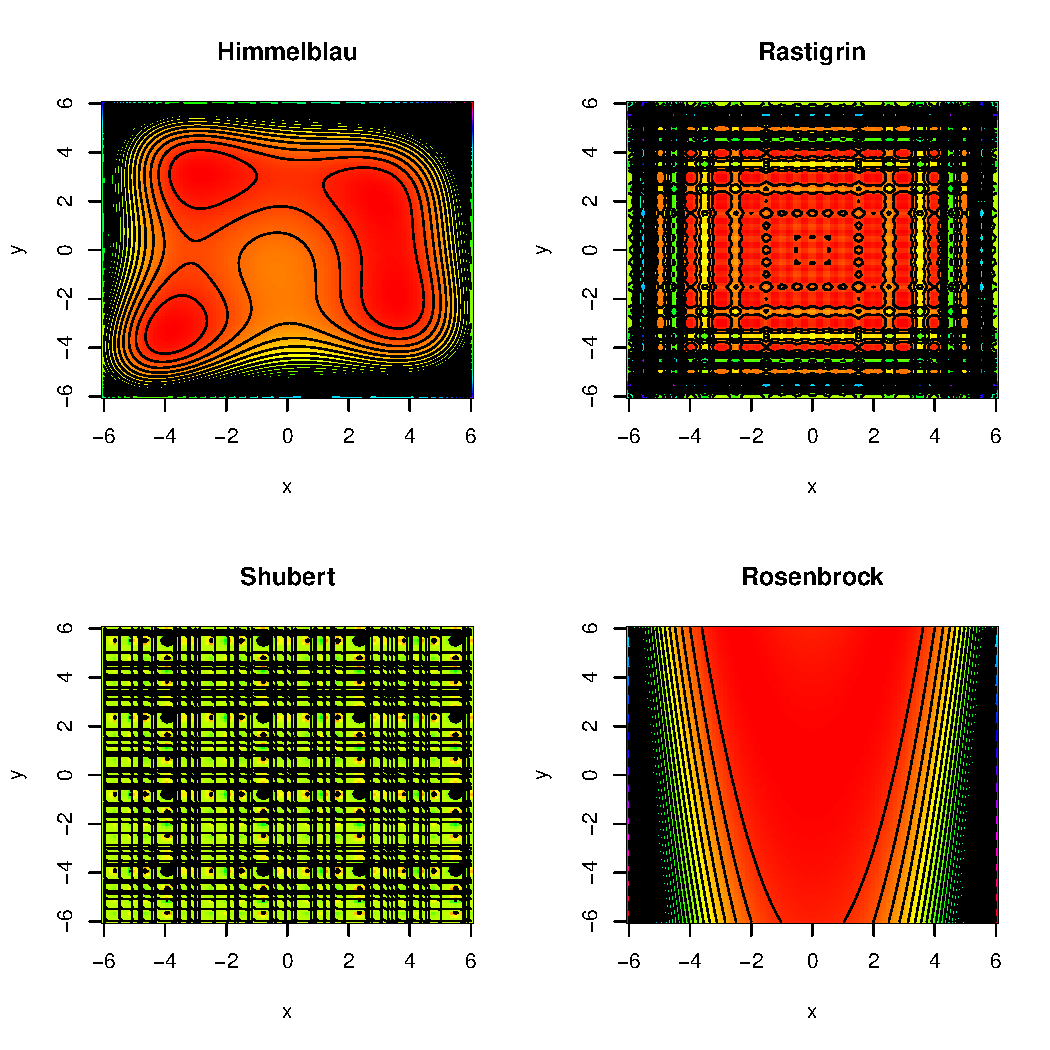
\includegraphics[height=3in,width=\textwidth]{john-plot-new3.pdf}
\caption{Test Functions.}
\end{figure}

\end{frame}
%%%%%%%%%%%%%%%%%%%%%%
\begin{frame}


\begin{figure}[hbp]
%\vspace{-1in}
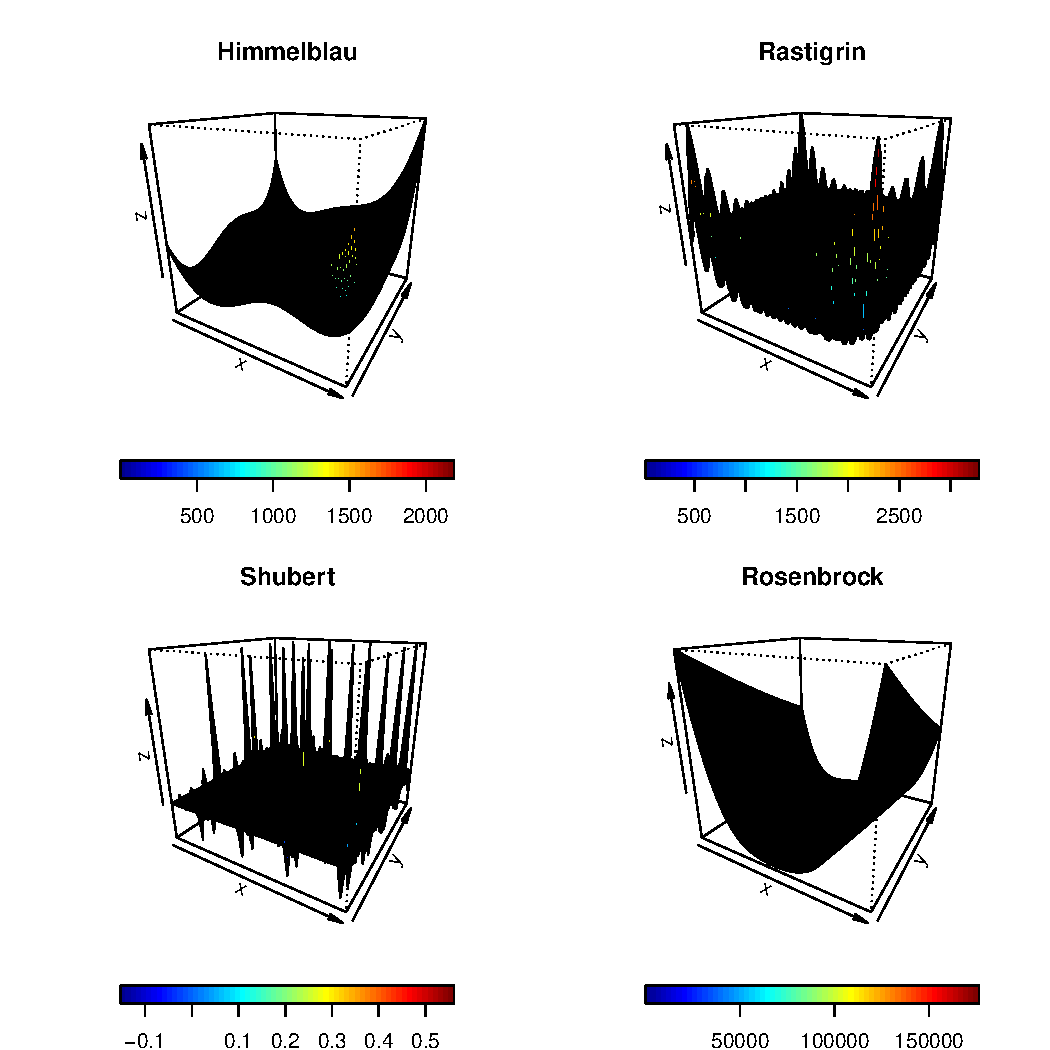
\includegraphics[height=3in,width=\textwidth]{john-plots-1.pdf}
\caption{Test Functions.}
\end{figure}

\end{frame}
%%%%%%%%%%%%%%%%
\begin{frame}
\frametitle{Basic Set-Up}


\footnotesize
\begin{itemize}
\item Find $ {\rm arg min}_x f(x)$ where $ x \in \mathcal{X} $ for a given objective function.

Possibility of multi-modality
$$
\mathcal{X}_{min} = \{  x \in \mathcal{X} : f( x) = \min_y f(y) \} \; .
$$
\item Duality with the problem of finding the modes of the Gibbs distribution with potential $f(x)$, indexed by a one-dimensional ``temperature'' parameter $\kappa$,
with density defined by
$$
\pi_\kappa (x) = \exp \left \{ - \kappa f(x) \right \} / Z_\kappa \; \; {\rm for} \; \; x \in \mathcal{X} \; .
$$
where
$ Z_\kappa = \int_{\mathcal{X}}  \exp \left \{ - \kappa f(x) \right \} d x $ which is never needed.

\item The limiting cases, $ \kappa =0 , \infty$ both lead to a uniform measure but on different sets.
For $ \kappa =0 $, we have $ \pi_0 (x) $ as the uniform measure on $ \mathcal{X} $ and as $ \kappa \rightarrow \infty $
we have a uniform measure on the set $ \mathcal{X}_{min} $. Specifically, we have
$$
\lim_{ \kappa \rightarrow \infty } \pi_\kappa (x) = \pi_{\infty} ( x ) = | \mathcal{X}_{min} |^{-1} \delta_{ \mathcal{X}_{min} } (x)
$$
where $ \delta_x$ denotes Dirac measure
\end{itemize}
\normalsize

\end{frame}
%%%%%%%%%%%%%%%%%%%%%%%
\begin{frame}
\frametitle{Slice Sampling}

\footnotesize
\begin{itemize}
\item Let $u$ be an auxiliary ``slice-variable'' and defining a joint distribution $ \pi(x,u)$ that is uniform
on the set $ U = \{ ( x , u) : 0 < u < \pi(x) \} $.

Therefore, $ p ( x , u) = 1 / Z $ on $U$ and zero otherwise. $ Z = \int_{\mathcal{X}} \pi(x ) d x $ is the appropriate normalisation constant.
\item The marginal is the desired normalised density as
$$
\pi(x) = \int_U \pi(x,u) d u = (1 / Z ) \int_0^{\pi(x)} d U = \pi(x)/Z  \; .
$$
Sample uniformly from the ``slice'' region defined by $u$, namely
$ \mathcal{S}_u = \{ x : u < \pi(x) \} $.

Convergence depends on the geometry of this set.
\item
A simple Gibbs sampler which iterates between drawing a uniform $ (u|x) \sim Uni ( 0, \pi(x) ) $
and $ (x|u) \sim Uni_{ \mathcal{S}_u } ( x ) $
\end{itemize}
\normalsize

\end{frame}
%%%%%%%%%%%%%%%%%%%%%%
\begin{frame}
\frametitle{Exponential Slice Sampling}

\footnotesize
\begin{itemize}
\item Additive function of interest $ f(x) = \sum_{i=1}^K f_i (x) $
$$
\pi_\kappa ( x ) = \exp \left ( - \kappa f (x) \right )/ Z_\kappa  = \exp \left ( - \kappa \sum_{i=1}^K f_i (x) \right ) / Z_\kappa \;.
$$
\item Define an auxiliary slice  variable $ (y | \kappa ) \sim Exp ( \kappa )$ such that
$$
\pi_\kappa (  x , y ) \propto p(y|\kappa) \mathbb{I}\left ( 0 \leq y \leq f(x) \right )
$$
\item
The appropriate marginal distribution, we have
$$
\pi_\kappa ( x , y ) \propto e^{ - \kappa y } \mathbb{I}\left ( 0 \leq y \leq f(x) \right )
$$
Integrating out $y$,
$$
\pi( x )  \propto \int_{f(x)}^\infty \kappa e^{-\kappa y} d y = \exp \left ( - \kappa f (x) \right )
$$
\item Simple Gibbs sampler
\begin{align*}
\pi( x|y ) & \propto \mathbb{I}\left ( f(x) \geq y \right ) =  \mathbb{I}\left ( x \in f^{-1} ( y ) \right )  \\
\pi( y|x ) & \propto e^{-\kappa y} \mathbb{I}\left ( y \leq f(x) \right ) \; .
\end{align*}
\end{itemize}
\normalsize

\end{frame}
%%%%%%%%%%%%%%%%%%%%%%%%%%%%%
\begin{frame}
\frametitle{Rosenbrock function}

\footnotesize
\begin{itemize}
\item
Find the minimum $(x_1,x_2)=(1,1)$ of the Rosenbrock function
$$
( 1- x_1 )^2 + c(x_2-x^2_1)^2 \; \; {\rm with} \; \; c = 100
$$
\item
Define the annealed distribution
$$
\pi_{\lambda} ( x_1 ,x_2) \propto \exp \left ( - \kappa \left \{ ( 1- x_1 )^2 + c(x_2-x^2_1)^2 \right \} \right )
$$
Slice-out the last term and set $ \kappa \in \{ 1 , 5 , 50 , 5000 \} $.
\item
Let $ ( u|x_1,x_2) \sim Uni \left (0, \exp \left \{ -  \kappa c (x_2-x^2_1)^2 \right \} \right ) $.

Then we have a three variable joint distribution
$$
\pi_{\kappa , \lambda} ( x ,y , u )  \propto \exp \left \{ - \kappa ( 1- x_1 )^2 \right \}
 \mathbb{I} \left ( 0 \leq u \leq \exp \left \{ - \kappa c (x_2-x^2_1)^2 \right \} \right )
$$
\end{itemize}
\normalsize

\end{frame}
%%%%%%%%%%%%%%%%%%%%%%
\begin{frame}
\frametitle{Conditionals}

\footnotesize
\begin{itemize}
\item
This has complete conditionals
\begin{align*}
\pi ( x_2 | x_1 ) & \sim \mathcal{N} ( x^2_1 , 2 / c \kappa  )\\
  \pi ( x_1 | x_2,u ) & \sim \mathcal{N} ( 1 , \kappa  ) \mathbb{I} \left ( a(u,x_2) \leq x \leq b(u,x_2) \right )\\
\pi ( u | x_1 , x_2 ) & \sim Uni \left (0, \exp \left \{ - \kappa c (x_2-x^2_1)^2 \right \} \right )
\end{align*}
This is a partially collapsed Gibbs sampler -- $ x_2 | x_1 $ and not $ x_2 | x_1 , u $.

\item
We find the constraint region $(a(u,y), b(u,y)) $ by inverting the slice region
$$
u \leq \exp \left \{ - \kappa c (x_2-x^2_1)^2 \right \} \; {\rm implies} \; x_2 - \sqrt{ - \ln u / \lambda} \leq x^2_1 \leq  x_2 + \sqrt{ - \ln u / \lambda}
$$
For $b>0$ and $ a \leq x^2_1 \leq b$ we have $ - \sqrt{a} \leq x_1 \leq \sqrt{b} $ we have
$$
a( u, x_2 ) = - \sqrt{ x_2 - \sqrt{ - \ln u / \lambda} } \; {\rm and} \; b( u, x_2 ) = \sqrt{ x_2 + \sqrt{ - \ln u / \lambda} }
$$
\end{itemize}
\normalsize
\end{frame}
%%%%%%%%%%%%%%%%%%%%%%
\begin{frame}


\begin{figure}[hbp]
%\vspace{-1in}
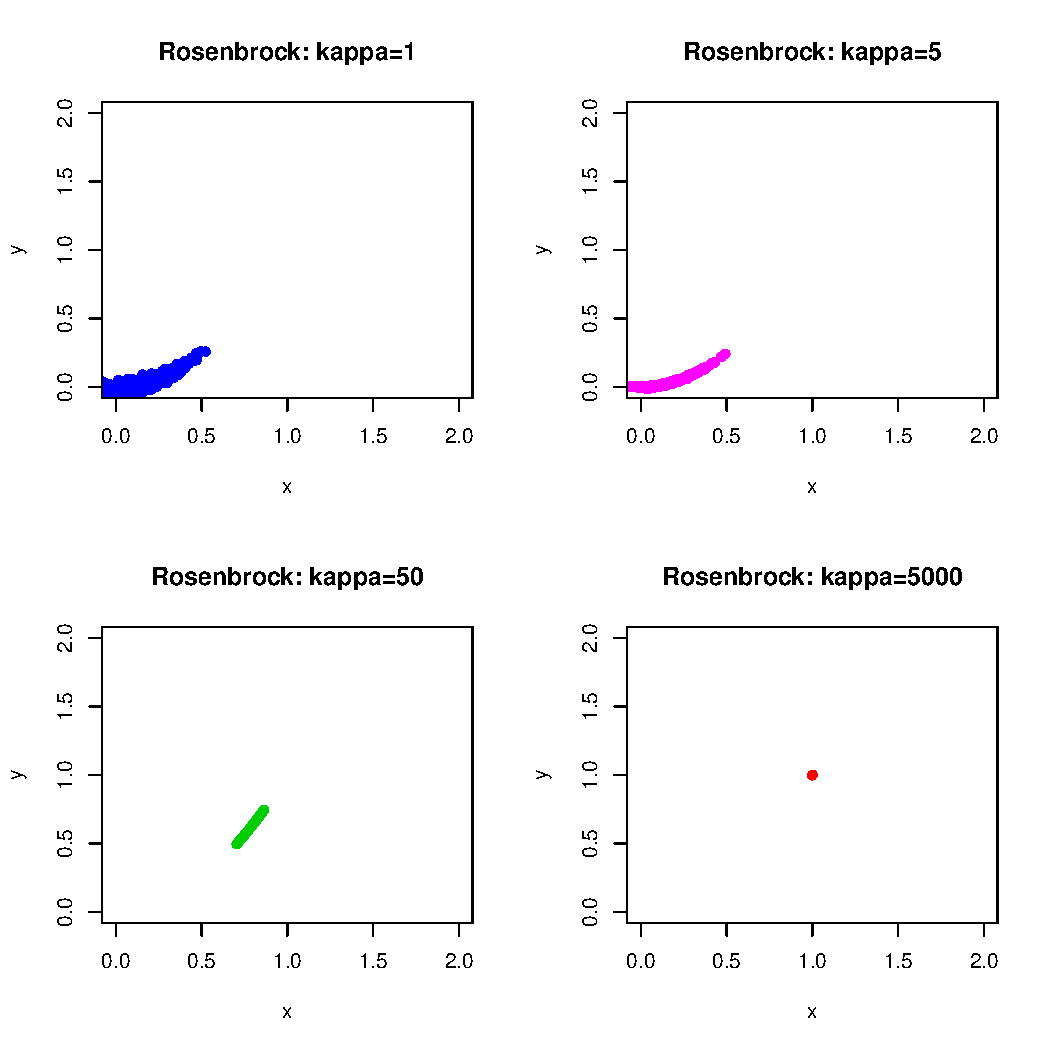
\includegraphics[height=3in,width=\textwidth]{john-rosen.pdf}
\caption{Rosenbrock.}
\end{figure}

\end{frame}
%%%%%%%%%%%%%%%%%%%%%%%%%
\begin{frame}
\frametitle{Himmelblau's function}

\footnotesize
\begin{itemize}
\item
Four identical local minima at zero and a local maximum at $ x_1=-0.27, x_2=-0.92 $.
$$
f(x_1,x_2) =  ( x^2_1 + x_2 - 11 )^2 + (  x_1 + x_2^2 - 5 )^2
$$
Minima are at $ (3,2) , (-2.805, 3.131 ), (-3.779 , -3.282) , (3.584 , -1.848 ) $.
\item
Annealed joint distribution
$$
\pi ( x_1 , x_2 ) \propto \exp \left \{ - \frac{\kappa}{2} \left (  ( x^2_1 + x_2 - 11 )^2 + (  x_1 + x_2^2 - 5 )^2 \right ) \right \}
$$
\item
Augment with two slice variables $ u_1, u_2 $
$$
\pi ( x_1 , x_2 ) \propto \mathbb{I} \left ( 0 \leq u_1 \leq \exp \left \{ - \frac{\kappa}{2} ( x^2_1 + x_2 - 11 )^2 \right \} \right )
 \mathbb{I} \left ( 0 \leq u_2 \leq \exp \left \{ - \frac{\kappa}{2} (  x_1 + x_2^2 - 5 )^2  \right \} \right )
$$
\end{itemize}
\normalsize
\end{frame}
%%%%%%%%%%%%%%%%%%%%%%
\begin{frame}

\footnotesize
\begin{itemize}
\item
We can invert the slice regions  as follows:
$$
- 2 \kappa^{-1} \log u_1 \geq  ( x^2_1 + x_2 - 11 )^2 \; \; {\rm and} \; \; - 2 \kappa^{-1} \log u_2 \geq  ( x_1 + x_2^2 - 5 )^2
$$
Therefore, for $(x_1|x_2)$ we have
\begin{align*}
a_x = 11 - x_2 - \sqrt{ - 2 \kappa^{-1} \log u_1 } & \leq x^2_1 \leq  11 - x_2 + \sqrt{ - 2 \kappa^{-1} \log u_1 } =b_x\\
c_x = 5 - x_2^2 - \sqrt{ - 2 \kappa^{-1} \log u_2 }& \leq x_1 \leq  5 - x_2^2 + \sqrt{ - 2 \kappa^{-1} \log u_2 } =d_x
\end{align*}
\item
For $(y|x)$ we can argue in a similar fashion to get
\begin{align*}
a_y = 5 - x_1 - \sqrt{ - 2 \kappa^{-1} \log u_1 } & \leq y^2 \leq  5 - x + \sqrt{ - 2 \kappa^{-1} \log u_1 } =b_y\\
c_y = 11 - x_1^2 - \sqrt{ - 2 \kappa^{-1} \log u_2 }& \leq y \leq  11 - x^2 + \sqrt{ - 2 \kappa^{-1} \log u_2 } =d_y
\end{align*}
The set of complete conditionals is then given by
\begin{align*}
\pi( x_1| x_2 , u_1 , u_2 ) & \sim Uni \left ( \max \left (  - \sqrt{ | a_x| } ,c_x \right ) , \min \left ( \sqrt{b_x} , d_x \right ) \right )\\
\pi( x_2| x_1 , u_1 , u_2 ) & \sim Uni \left ( \max \left (  - \sqrt{ | a_y| } ,c_y \right ) , \min \left ( \sqrt{b_y} , d_y \right ) \right )\\
\pi( u_1 | x_1, x_2 ) & \sim Uni \left ( 0 , \exp \left \{ - \kappa ( x^2_1 + x_2 - 11 )^2 \right \} \right ) \\
\pi( u_2 | x_1 , x_2) & \sim Uni \left ( 0 , \exp \left \{ - \kappa ( x_1 + x_2^2 - 5 )^2 \right \} \right )
\end{align*}
\end{itemize}
\normalsize

\end{frame}
%%%%%%%%%%%%%%%%%%%%%%
\begin{frame}

\begin{figure}[hbp]
%\vspace{-1in}
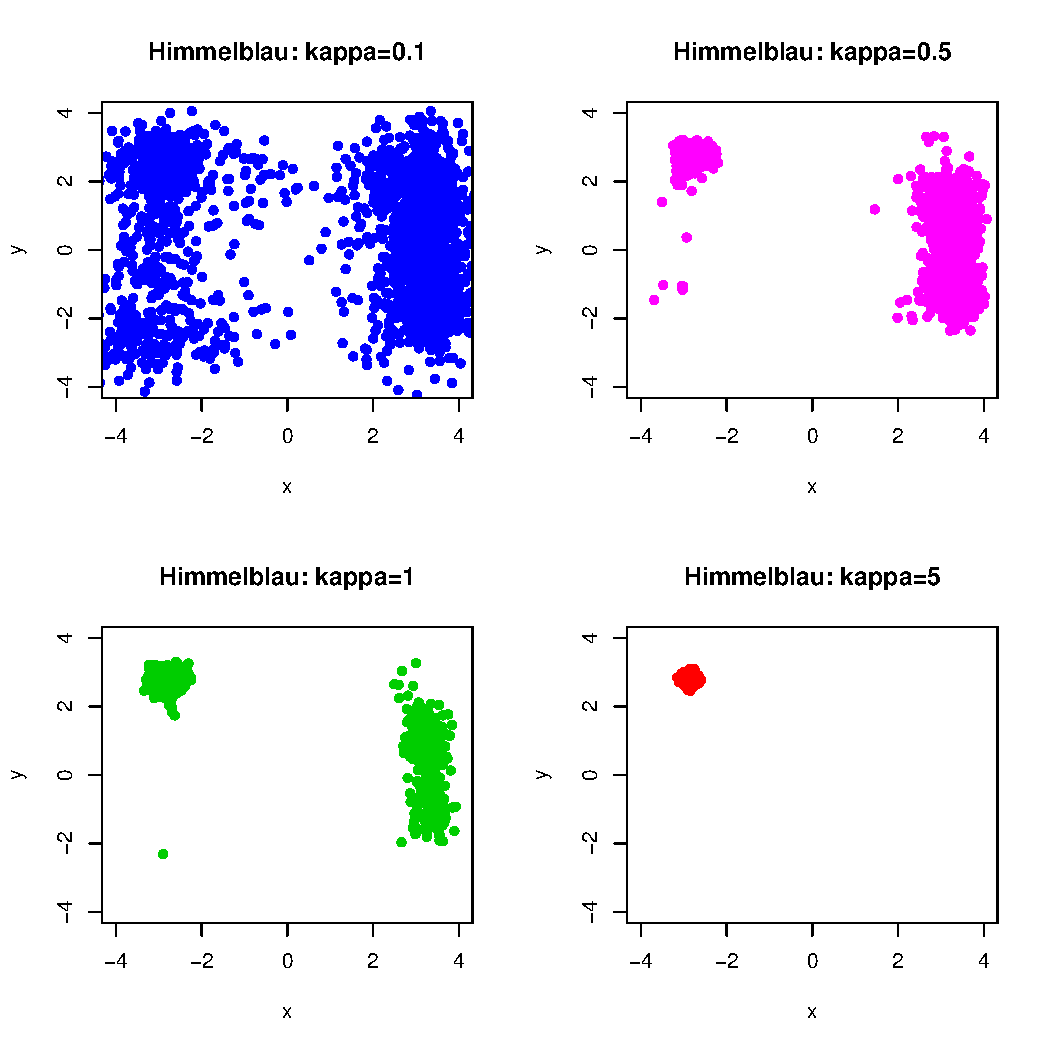
\includegraphics[height=3in,width=\textwidth]{john-himmelblau.pdf}
\caption{Himmelblau.}
\end{figure}

\end{frame}
%%%%%%%%%%%%%%%%%%%%%%
\begin{frame}
\frametitle{Rastigrin}

\footnotesize
The Rastigrin function with a global minimum at $ (0,0)$
$$
f( x ) = A k + \sum_{j=1}^k \left ( x_j^2 - A cos ( 2 \pi x_j ) \right )
$$
\begin{itemize}
\item Annealed Gibbs distribution
$$
\pi_\kappa ( x ) \propto e^{ - \kappa f( x ) } = \exp \left \{ - \kappa \sum_{j=1}^K x_j^2 \right \}
 \exp \left \{ \kappa A \sum_{j=1}^k  cos ( 2 \pi x_j ) \right \}
$$
\item
Exponential sliced joint distribution
$$
 \pi_\kappa ( u_1 , \ldots , u_k , x_1 , \ldots ,x_k  ) \propto \exp \left \{ - \kappa \sum_{j=1}^k x_j^2 \right \}
\mathbb{I} \left ( - \kappa A cos (2 \pi x_j ) \leq u_j  \right ) e^{- u_j}
$$
The slice region is easy to invert
$ x_j \leq (2 \pi)^{-1} cos^{-1} \left ( - u_j /A \kappa \right ) $.
\item
Gibbs sampler with the conditionals, for $ 1 \leq j \leq K $
\begin{align*}
\pi_\kappa ( x_j | u , x_{-j} ) & \sim \mathcal{N} \left ( 0 , (2J)^{-1} \right )
 \mathbb{I} \left ( x_j \leq (2 \pi)^{-1} cos^{-1} \left ( - u_j /A \kappa \right )  \right )\\
\pi_\kappa ( u_j | x_j  ) & \sim \mathcal{E} [ - \kappa A cos (2 \pi x_j ) , \infty )
\end{align*}
\end{itemize}
\normalsize

\end{frame}
%%%%%%%%%%%%%%%%%%%%%%%%%
\begin{frame}

\begin{figure}[hbp]
%\vspace{-1in}
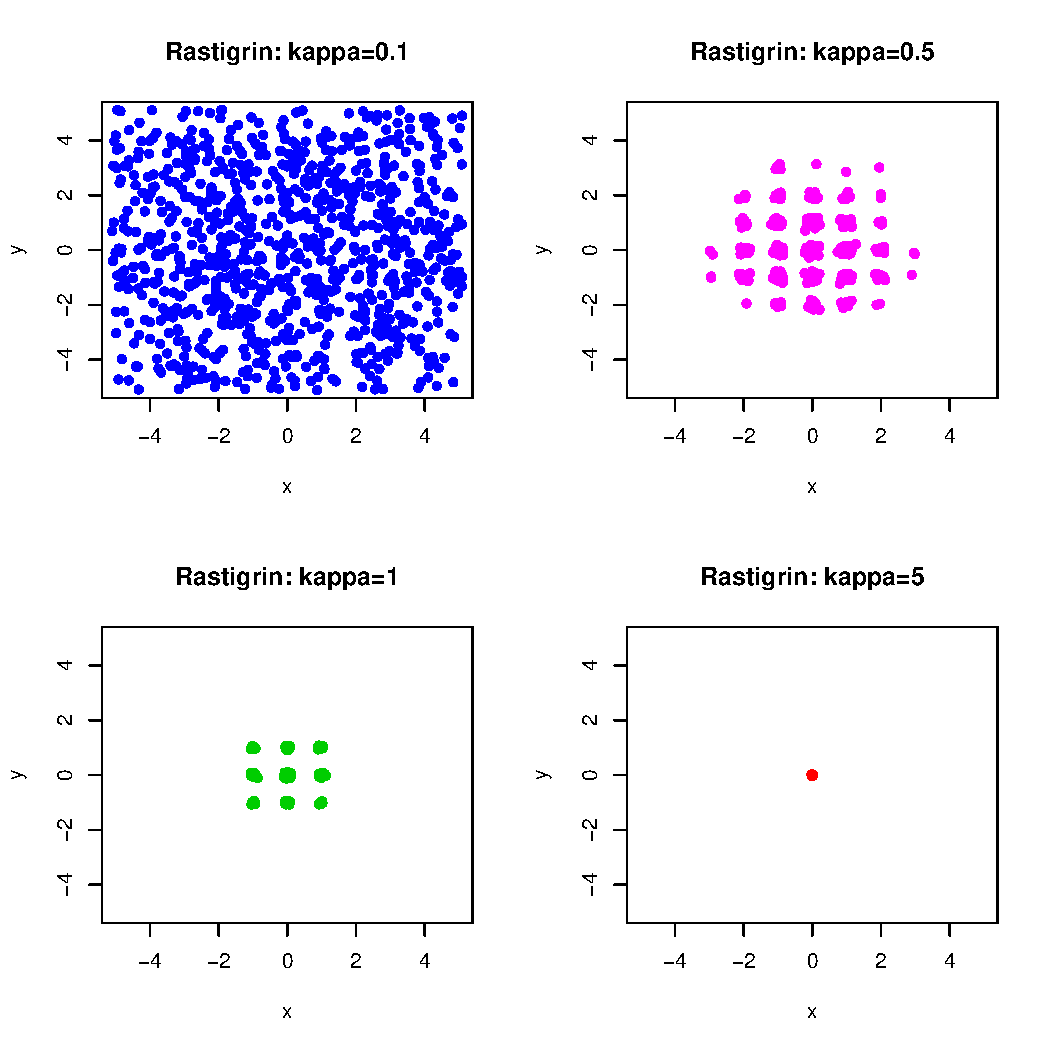
\includegraphics[height=3in,width=\textwidth]{john-rastigrin.pdf}
\caption{Rastigrin.}
\end{figure}

\end{frame}
%%%%%%%%%%%%%%%%%%%%%%%%%%%
\begin{frame}
\frametitle{Shubert Function}

\footnotesize
The Shubert function is  $ f( x ) = \sum_{j=1}^5 j cos \left ( ( j+1 ) x + j \right ) $ with annealed density
$$
\pi_\kappa ( x_1 , x_2 ) = \exp \left ( - \kappa f( x_1 ) f( x_2 ) \right ) / Z_\kappa
$$
\begin{itemize}
\item
The conditional $ \pi_\kappa ( x_1 | x_2 )$ can be written as
$$
 \pi_\kappa ( x_1 | x_2 ) = \prod_{j=1}^5 \exp \left \{ - f( x_2 ) j cos \left ( (j+1) x_1 + j \right ) \right \}
$$
Consider the slice joint distribution that is a conditional uniform
$$
 \pi_\kappa ( u_1 , \ldots , u_J , x_1 | x_2 ) \propto \mathbb{I}
 \left ( 0 \leq u_j \leq e^{ - C( x_2 ) j cos \left ( (j+1) x_1 + j \right ) } \right )
$$
Invert
$ (j+1) x_1 + j \leq cos^{-1} \left ( \frac{1}{j} \ln \frac{u_j}{C(x_2)} \right ) $.
\item
Run a Gibbs sampler with the conditionals, for $ 1 \leq j \leq K $
\begin{align*}
\pi_\kappa ( x_1 | u , x_2 ) & \sim \mathcal{U} \\
\pi_\kappa ( u_j | x_1  ) & \sim \mathcal{U} \left ( 0 \leq u_j \leq e^{ - C( x_2 ) j cos \left ( (j+1) x_1 + j \right ) } \right )
\end{align*}
A $12$ dimensional Gibbs sampler.
\end{itemize}
\normalsize

\end{frame}
%%%%%%%%%%%%%%%%%%%%%%
\begin{frame}

\begin{figure}[hbp]
%\vspace{-1in}
\includegraphics[height=3in,width=\textwidth]{john-shubert.pdf}
\caption{Shubert.}
\end{figure}

\end{frame}
%%%%%%%%%%%%%%%%%%%%%%
\begin{frame}
\frametitle{Discussion}

\footnotesize
Optimization via Simulation

\begin{itemize}
\item A variety of shapes and surfaces:

Himmelblau, Rastigrin, Rosenbrock, Shubert

\item Exponential Slice Sampler

Good ergodic properties even though higher dimensionality -- depends on the geometry of the slice-set

\item Other strategies: Simulated tempering; equi-energy sampler; Wang-Landau algorithm.

\end{itemize}
\normalsize

\end{frame}
%%%%%%%%%%%%


%%%%%%%%%%%%%%%%%%%%%%%%%%
\end{document}


\section{Introduction}

Optimisation of complex multi-modal objective functions involves many challenges.
There is a well-known duality with simulated annealing procedures for finding the mode of the associated Gibbs distribution defined
with the given objective function as its potential.
To illustrate our methodology, we consider four classic global optimisation test functions;
the Rosenbrock, Himmelblau, Rastigrin and Shubert functions.
Figures 1 and 2 show contour and drape-plots of these functions.
Clearly, this set of functions exhibits a variety of challenges: a global mode in a long valley (Rosenbrock),
multiple local and one global mode (Rastigrin) to multi-modality (Himmelblau, Shubert). Traditional derivative-based methods can clearly have difficulties.
For example, even in the Rosenbrock function, gradient-based methods can have difficulty in finding the solution at the end of a long steep valley.
For a method to be successful it needs to be able to scale to this multitude of different function types without resorting to extra information.

Markov chain simulation methods are adaptive approach to the problem.
They have the advantage of being derivative-free. In this paper, we propose a new Markov chain simulation method based on exponential slice sampling
of the associated Gibbs distribution defined by the objective function of interest.
We show that our approach extends to additive functions and leads to a slice sampling algorithm that can be viewed within the Swendsen-Wang algorithmic framework
(Edwards and Sokal, 1988). There are a number of other popular simulation-based methods ranging
from simulated annealing (Kirkpatrick et al, 1983, Geman, 1990),
direct and evolutionary Metropolis MCMC (Liu, et al, 2000), particle swarm (Kennedy and Eberhart, 1995), multi-set sampling (Leman, Chen and Lavine, 1999)
and stochastic guided search (Gramacy and Taddy, 2010, Taddy, Lee, Gray and Griffin, 2008). Janson and Middendorf (2005) illustrate the use of particle swarm methods on the
Rosenbrock and Rastigrin functions.

The Gibbs distribution associated with the objective function is defined by a one-parameter exponential family of the form

Pincus (1968, 1970) and Geman (1990) proposed the use of simulation-based Metropolis-Hastings (MCMC) algorithms to sample and find the modes of this distribution.
For very complex functions, directly applying MCMC methods can be fraught with convergence difficulties as the sampler can easily get stuck in the local modes
and careful tuning of algorithms for specific cases is generally required.
One advantage of our approach is that we introduce no further tuning parameters (step sizes etc) other than the traditional cooling
parameter $\kappa$ that's used in defining the Gibbs distribution. We follow the simulated tempering literature by focusing on a set
of pre-determined values $ 0 < \kappa_1 < \ldots < \kappa_m $ rather than using a cooling ``schedule'' as in simulated annealing (SA).
The limiting properties as $\kappa \rightarrow \infty $ still hold for our sampler -- but the key insight of
our slice sampler is that it provides a Markov chain that has good ergodic properties (even with as few as $1000$ draws for the objective functions
considered here) and that convergence at low values
of $\kappa$ is sufficient for the chain to traverse even the most complicated of functions.

The rest of the paper is as follows. Section 2 describes our simulation-based optimisation procedure. It develops the exponential slice sampler
and the extension to additive functionals and the Swendsen-Wang algorithm.
Section 3 illustrates our method on the Himmelblau, Rastigrin, Rosenbrock
and Shubert functions. We show how to calculate the slice-set for each of the functions in turn. One of the advantages of our approach
is that it doesn't require additional tuning. We use the same set of cooling temperatures except for the Rosenbrock function which needs more cooling
due to its long ridge. In all cases our
slice sampling algorithm converges quickly to equilibrium, in line with theoretical results (Tweedie and Mengersen, 1994, Polson, 1996,
Roberts and Rosenthal, 1999). Finally, Section 4 concludes with directions for future research.

\section{Simulation-based Optimisation via Slice Sampling}

is
the normalisation constant, or partition function. Like simulated tempering, we have to perform a sensitivity analysis with respect to
the cooling parameter $\kappa$ by specifying an initial set of values.

We will use Markov chain MC simulation methods to sample from this
possibly high dimensional joint distribution. One advantage of this approach is that they  will not be require explicit knowledge of $Z_\kappa $.
There are, however, many possible Markov transition dynamics that have the appropriate equilibrium distribution.
Here we propose a new method based on exponential slice sampling.

The limiting cases, $ \kappa =0 , \infty$ both lead to a uniform measure but on different sets.
For $ \kappa =0 $, we have $ \pi_0 (x) $ as the uniform measure on $ \mathcal{X} $ and as $ \kappa \rightarrow \infty $
we have a uniform measure on the set $ \mathcal{X}_{min} $. Specifically, we have
$$
\lim_{ \kappa \rightarrow \infty } \pi_\kappa (x) = \pi_{\infty} ( x ) = | \mathcal{X}_{min} |^{-1} \delta_{ \mathcal{X}_{min} } (x)
$$
where $ \delta_x$ denotes Dirac measure.  See Azencott (1988) for further discussion.

The asymptotic in $\kappa $ is the basis of simulated annealing (Kirkpatrick et al, 1983, Aarts and Korst, 1988, Van Laarhoven and Aarts, 1987)
which uses a schedule of parameter values $ \kappa^{(g)} $ that increases with the length of the Markov chain simulation in an appropriate fashion (Gidas, 1985).
Other approaches include simulated tempering (Marinari and Parisi, 1992, Geyer and Thompson, 1995) which uses a random walk on a set of
temperature values $ 0 < \kappa_1 < \ldots < \kappa_m $ rather than increasing $\kappa$ on a schedule, equi-energy sampling (Kou, Zhou and Wong, 2006), evolutionary
MCMC (Liu, Liang and Wong, 2000, 2001) and the Wang-Landau algorithm (Atchade and Liu, 2010).

There are a number of ways of computing the mode: for example, the use Markov chain
simulation methods. For a fixed $\kappa$, consider running Markov chain $ X^{(0)} , X^{(1)} , \ldots , X^{(G)} , \ldots $
with a transition kernel defined so as to have the appropriate equilibrium distribution $ \pi_\kappa (x)$. Then under mild Harris recurrence conditions,
given any starting point,
$$ \lim_{ G \rightarrow \infty} \mathbb{P} \left ( X^{(G)} \in A | X^{0)}= y \right ) = \pi_\kappa (A )
$$
for any Borel sets $A$,
see Tierney (1994) for further discussion. The main issue is which Markov chain to use? We will argue for the use of slice sampling methods
for a set of temperature values defined in a given set in a similar fashion to simulated tempering.


In seminal work, Pincus (1968, 1970) proposed to directly use a Metropolis algorithm to simulate from
the Gibbs distribution, then after discarding a burn-in period, to use the ergodic mean along the chain $ \frac{1}{G} \sum_{g=1}^G X^{(g)} $ as an estimate of the mode.
In the uni-modal case, as $ \kappa \rightarrow \infty $, this will find the mode. The simulated annealing literature
also includes $ \kappa $ as a control parameter in the Markov chain, which indexes the transition kernel with $ \kappa^{(g)} $.
This now makes the simulation procedure a time-inhomogeneous chain and conditions on the choice of schedule $ \kappa^{(g)} $ are
required to guarantee convergence to the mode, see Gidas (1985) and Geman (1990) for further discussion.

We note that even in the multimodal case,  a suitably defined Markov chain will converge
to a uniform measure over the modes and by monitoring the output of the chain, in principle we can find all the modes.
On the theoretical side, the issue is where the constructed Markov chain converges in polynomial time so that the conductance (Polson, 1996)
of moving from mode to mode for a large $\kappa$ is high enough. Clearly, in hard multi-modal cases this is unlikely to be the case, as
the surfaces typically have witches' hat spikes (Geyer, 1992, Polson, 1992) where it is known that even though there is geometric
convergence of a simple Gibbs sampler it is not polynomial.

Therefore, from purely practical reasons, we adopt a slightly different approach.
We propose to use slice sampling.  This requires a priori knowledge of the function and as we will see computation of ``slice sets''.
By defining a Markov chain in higher dimensions with the use of auxiliary slice variables, we can exploit the convergence properties of the slice sampler:
geometric (Roberts and Polson, 1994) and uniformly when $ \mathcal{X}$ is bounded and $ supp (f) < \infty $, see Mira and Tierney (2002).
Convergence is for the joint and that for the marginal on $x$ follows from that. This doesn't guarantee polynomial time convergence, as there still
might be a long icicle of probability in the convex set defined by the slice regions which makes it hard for a conditional Gibbs or Metropolis
algorithm to traverse. However, for many problems of interest this takes a spiking multi-modal surface which is not log-concave and hard to construct
a Markov chain that has good conductance properties to a far higher dimensional chain that has good convergence properties (see Polson, 1996).
Esseentially, we have put some volume back into the spiky regions -- and after the chain has converged in the higher dimensional set  we can
project the draws back down into the dimensions of interest. On the marginal set, the chain will have no difficulty in traversing the modes
particularly for lower values of $ \kappa $.

We also modify the standard uniform slice sampler and introduce the exponential slice sampler.
We show that for a wide range of test functions that empirical this performs well.


\subsection{Slice Sampling}

The intuition behind uniform slice sampling is simple. Suppose that we wish to sample from a possible high dimensional un-normalised density
$ \pi(x) $. We do this by sampling uniformly from the region that lies under the desnity flot of $\pi$. This idea is formalised
by letting  provides a Markov chain with the appropriate joint distribution $\pi(x,u)$ and hence marginal
$ \pi(x)/Z$.

This is a special case of the so-called Swenden-Wang algorithm (Edwards and Sokal, 1988). Suppose that we wish to
sample from a density that is a product of functions: $p(x) = \pi_1 (x ) \ldots \pi_K (x) / Z_K $. Then we introduce
a set of $K$ auxiliary uniform slice variables $ (u_1 , \ldots , u_K )$ and
a joint $(x, u_1 , \ldots, u_K )$ that is uniform on the ``slice'' region:
$$
 \mathcal{S}_u = \{ x : u_i < \pi(x) \; \; \forall i \; \}
$$
Then we sample in a Gibbs fashion, from the complete conditionals
$$
(u_i | x ) \sim Uni ( 0, \pi_i(x) ) \; {\rm for} \;  i = 1 , \ldots , K  \; \; {\rm  and} \;  \; (x|u) \sim Uni_{ \mathcal{S}_u } ( x ) \; .
$$

For ease of implementation, we have to be able to compute the slice set and the  set-theoretic inverse $f^{-1}$.
We also need to be able to sample from a truncated version of $f$ and from a truncated exponential.

There are a number of extensions of this algorithm. First, suppose that we wish to sample from
$ \pi_\kappa (x ) = g(x) \exp \left ( - \kappa f(x) \right ) / Z_\kappa $ where $ g(x) $ and its truncated counterpart are straightforward to sample (Devroye, 1986).
Then we can slice the last term and consider the augmented joint distribution
$$
 \pi_\kappa (x, y ) = g(x) e^{ - \kappa y } \mathbb{I}\left ( 0 \leq y \leq f(x) \right )
$$
In a similar fashion this leads to a simple Gibbs sampler with the only difference being that we have to draw from $g(x)$ on the conditioned slice set given $y$.

Second, by introducing multiple exponential slice variables, as in the Swendsen-Wang algorithm, we extend this to densities of the form
$$
\pi_\kappa ( x ) = \exp \left ( - \kappa \sum_{i=1}^K f_i (x) \right ) / Z_\kappa
$$
The advantage of our approach is that it works seamlessly for large values of $K$. Hence we can deal efficiently with multi-modal functions.

Specifically,  define multiple independent exponential slice variables $y_1 , \ldots , y_K $ and a joint distribution
$$
\pi(  x , y_1 , \ldots , y_k ) = \exp \left ( - \kappa \sum_{i=1}^K y_i \right ) \prod_{i=1}^K \mathbb{I}\left ( 0 \leq y_i \leq f_i(x) \right ) / Z_\kappa
$$
For the $ p( x | y_1 , \ldots , y_K )$ conditional we now need to sample from
$$
\pi( x|y )  \sim Uni \left \{   f_i(x) \geq y_i \; \forall i \;  = \cup_{i=1}^K \left ( x_i \in f^{-1}_i ( y_i ) \right ) \right \}
$$
Neal (2003) for a general approach for dealing with sets of this form.

Finally, we can use the first coordinate of the draws from the joint distribution as a sample from the marginal dustribution
$\pi_\kappa (x)$ of interest.
So far we have constructed a Markov chain that generates a sequence of draws $\left ( x^{(n)} , y_1^{(n)} , \ldots,  y_k^{(n)} \right ) $
which converges in distribution as $ n \rightarrow \infty $ to a draw $( x , y_1 , \ldots , y_k) \sim \pi $ from the joint distribution of interest.
We write
$ \left ( x^{(n)} , y_1^{(n)} , \ldots , y_k^{(n)} \right ) \stackrel{D}{=} ( x , y_1,\ldots ,y_k ) \sim \pi $.
Given standard properties of weak convergence (or convergence in distribution), we have weak convergence for functionals $F: \Re^K
\rightarrow \Re^p $ where $ p \leq K $ and we have
$$
F \left ( x^{(n)} , y_1^{(n)} , \ldots , y_k^{(n)} \right ) \stackrel{D}{=} F ( x , y_1,\ldots , y_k ) \; .
$$
We can use this to estimate means $ \mathbb{E}_\pi \left ( g ( x ) \right ) $ of posterior functionals of interest by appealing to the ergodic theorem and using a delayed average mean estimator $ \frac{1}{N} \sum_{n=1}^N f( X^{(n)} ) $
along the dependent draws of the chain.

This approach can also be uses to perform marginal density estimation. Suppose that we require an estimator $ \hat{\pi}(x) $ of
Given $ F ( x, y_1,\ldots , y_k ) = x $. Therefore, we have $ x^{(n)} \stackrel{D}{=}  x $ as
$ n \rightarrow \infty $.  We can  average along the chain to obtain the histogram density estimator
of the marginal distribution
$$
\hat{\pi} ( x )= \frac{1}{N} \sum_{n=1}^N \delta_{ x^{(n)} } ( x )
$$
where $ \delta_x ( \cdot) $ is the Dirac measure at point $x$.

This is the so-called marginalised Rao-Blackwell density estimate if we replace the Dirac measure by $\pi(x|y_1 ,\ldots , y_k)$.

\section{Four Examples}

All these problems require the minimisation of a bivariate additive objective function
$f(x)$ defined over a bounded region for $ x = \{ x_1 , x_2 \} \in \Re^2 $.
We apply our general exponential slice sampler as the  function are additive $ f(x_1,x_2) = \sum_{i=1}^K f_i(x_1,x_2) $.
We will apply our exponential slice sampler to the distribution
$$
\pi_\kappa ( x_1 , x_2 ) \propto \exp \left ( - \kappa \sum_{i=1}^K f_i(x_1,x_2) \right )
$$
First, as in simualted tempering, we have to define a set of temperatures $ 0 < \kappa_1 < \ldots < \kappa_m $ to run our Markov chain.
For all four example, we pick $m=4$ and take $ \kappa \in \{ 0.1, 0.5 , 1 , 5 \} $. From our empirical findings this set of values
is sufficient to traverse the behvaiour of all four functions without the need for further scaling.



\
If the autocorrelation is high then can also just use particle methods and re-sampling.

This is also related to the Rastigin function
$$
f(x) = A k + \sum_{j=1}^k \left ( x_i^2 - A cos ( 2 \pi x_i ) \right )
$$
with a global minimum at $ f(0,0)$. $A=10$ and $ -5.12 < x_i < 5.12 $.







\section{Discussion}

In our applications we will primilarly be interested in the bivariate case where
$ x^\star = ( x^\star_1 , x^\star_2) $ although our methods clearly extend to high dimensions and all allow for the possibility of
constraints (Geman, 1990).

There is another class of functions that can directly be sampled as either conditional normals or a bivariate normal.
One such function is the Booth Function:
$$
( x_1 + 2 x_2 - 7 )^2 + ( 2 x_1 + x_2 - 5 )^2
$$
which has a minimum at $ f(1,3) =0 $.
We can directly define a joint distribution
\begin{align*}
\pi ( x_1 , x_2) & \propto \exp \left \{ - \frac{\kappa}{2} \left ( ( x_1 + 2 x_2 - 7 )^2 + ( 2 x_1 + x_2 - 5 )^2 \right ) \right \}\\
& \propto \exp \left \{ - \frac{\kappa}{2}  \left ( 5 x^2_1 + 5 x^2_2 + 8 x_1 x_2 - 34 x_1 - 38 x_2 \right ) \right \}\\
 & \propto \exp \left \{ - \frac{\kappa}{2}  ( z - \mu )^\prime Q^{-1} ( z - \mu ) \right \}
\end{align*}
where $ z = (x_1 , x_2 ) $ and $ \mu = ( 1 , 3 ) $ and $ Q = \frac{1}{9} \left ( 5 , 4 ; - 4 , 5 \right ) $.

This is bivariate normal distribution -- clearly the minimum is $(1,3)$ and the density collapses on this as $ \kappa \rightarrow \infty $.

Metropolis has the advantage that it only needs the local difference $ f(x) - f(y) $ for the
density ratio $ \pi(x)/\pi(y)$. Hence it can be used for "black-box" functions.

The slice sampler is not the only data augmentation scheme that could be used. Whenever you can write
$$
\pi(x) = \mathbb{E} \left ( \pi( x , \omega ) \right )
$$
where $ \pi( x , \omega ) = p( x | \omega )p( \omega) $ we can simulate the joint $ \pi(x, \omega)$.
Typical examples include the class of $k$-monotone functions where $ p(x| \omega) $ is a Beta distribution.
The class of variance-mean mixtures leads to many of the well-known criterion functuions.

Constrained optimisation (Whittle, 1992, Birge and Louveaux, 1997, Mueller, 2000, Asmussen and Glynn, 2008) presents another class of challenges.
Within the sampling of the Gibbs distribution these can be added in a variety of ways, see for example Geman and Geman (1985).




\section{References}

\begin{description}
\item Aarts, E and Korst, J. (1989). \textit{Simulated Annealing and Boltzmann Machines}. Wiley, NY.

\item Atchade, Y. and J. Liu (2010). The Wang-Landau algorithm in general state spaces: applications and convergence analysis.
\textit{Statistica Sinica}, 20, 209-233.

\item Asmussen, S. and P. Glynn (2008). \textit{Stochastic Simulation}. Springer-Verlag, New York.

\item Azencott, R. (1988). Simulated Annealing. \textit{Seminaire Bourbaki}, 697.

\item Birge, J.R. and F. Louveaux (1997). \textit{Introduction to Stochastic
Programming}. Springer, New York.

\item Devroye, L. (1986). \textit{Non-uniform Random Variate Generation}, Springer Verlag, New York.

\item Edwards, R.G. and A.D. Sokal (1988). Generalisation of the Fortuin-Kastelyn-Swendsen-Wang algorithm.
\textit{Phys. Review D.}, 38(6), 2009-2012.

\item Geman, D. (1990).
\textit{Random Fields and Inverse Problems in Imaging}. Lecture Notes, Springer-Verlag, 113-193.

\item Geman, D. and S. Geman (1985). Relaxation and annealing with constraints.
\textit{Technical Report 35}, Brown University.

\item Geyer, C.J. (1992). Practical Markov chain Monte Carlo
(with discussion). \textit{Statistical Science }7, 473-511.

\item Geyer, C.J. and E.A. Thompson (1995). Annealing MCMC with applications to Ancestral Inference.
\textit{Journal of the American Statistical Association}, 90, 909-920.

\item Gidas, B. (1985). Nonstationary Markov chains and convergence of the annealing algorithm.
\textit{J. Stat. Phys.}, 39, 73-131.

\item Gramacy, R. and M. Taddy (2010). Categorical Inputs, Sensitivity Analysis, Optimization and Importance Tempering in {\tt tgp}.
\textit{J. Statistical Software}, 22(6), 1-48.

\item Janson, S. and M. Middendorf (2005). A Hierarchical Particle Swarm Optimiser and its Adaptive Variant.
\textit{IEEE Trans in Systems, Man, and Cybernetics}, 35(6), 1272-1282.

\item Kennedy, J. and R. Eberhart (1995). Particle Swarm Optimisation.
\textit{IEEE Int. Conf. on Neural Networks}, 1942-1948.


\item Kirkpatrick, S., C.D. Gelatt and M.P. Vecchi, (1983). Optimization by
simulated annealing, \textit{Science}, 220, 671-680.

\item Kou, S.C., Zhou, Q. and W.H. Wong (2006). Equi-Energy Sampler with applicationbs in statistical inference
and statistical mechanics (with Discussion). \textit{Annals of Statistics}, 34(4), 1581-1619.

\item Leman, S.C., Y. Chen and M. Lavine (2009). The Multi-Set Sampler.
\textit{Journal of the American Statistical Association}, 104, 1029-1041.

\item Liu, J.S., Liang, F. and W.H. Wong (2000). The Multiple-Try Method and Local Optimisation in
Metropolis Sampling. \textit{Journal of the American Statistical Association}, 95, 121-134.

\item Liu, J.S., Liang, F. and W.H. Wong (2001). A theory of dynamic weighting in Monte Carlo.
\textit{Journal of the American Statistical Association}, 96, 561-573.

\item Marinari, E. and G. Parisi (1992). Simulated Tempering: A Monte Carlo scheme.
\textit{Europhys Lett EPL}, 19, 451-458.

\item Mira, A. and L. Tierney (2002). Efficiency and Convergence Properties of Slice Samplers.
\textit{Scandinavian Journal of Statistics}, 29(1), 1-12.

\item Mueller, P. (2000). Simulation-Based Optimal Design.
\textit{Bayesian Statistics 6}, Bernardo et al eds, Oxford, 459-474.

\item Neal, R. (2003). Slice Sampling (with Discussion). \textit{Annals of Statistics}, 31(3), 705-767.

\item Park, T. and D.A. van Dyk (2008). Partially Collapsed Gibbs Samplers: Theory and Methods.
\textit{Journal of the American Statistical Association}, 103, 790-796.

\item Pincus, M. (1968). A Closed Form Solution of Certain Dynamic
Programming Problems. \textit{Operations Research}, 16, 690-694.

\item Pincus, M. (1970). A Monte Carlo Method for Approximate Solution
of certain types of Constrained Optimization Problems.
\textit{Operations Research}, 18, 6, 1225-1228.

\item Polson, N.G. (1992). Comment on Practical Markov chain
Monte Carlo by C. Geyer, \textit{Statistical Science}, 7, 490-491.

\item Polson, N. G. (1996). Convergence of Markov Chain Monte Carlo Algorithms.
\textit{Bayesian Statistics 5}, Bernardo et al eds, Oxford, 297-321.

\item Roberts, G.O.  and Polson, N. G. (1994). On the Geometric Convergence of the Gibbs Sampler.
\textit{J. R. Statist. Soc.}, B, 56, 2, 377-384.

\item Roberts, G.O.  and J. Rosenthal (1999). Convergence of slice sampler Markov chains.
\textit{J. R. Statist. Soc.}, B, 61, 643-660.


\item Taddy, M., H.K.H. Lee, G.A. Gray and J.D. Griffin (2009). Bayesian Guided Pattern Search for Robust Local Optimization.
\textit{Technometrics}, 51, 389-401.

\item Tibbits, M., M. Haran, J.C. Lietchy (2009). Parallel Multivariate Slice Sampling.
\textit{Technical Report}.

\item Tierney, L. (1994). Markov Chains for exploring Posterior
Distributions (with discussion). \textit{Annals of Statistics }22,
1701-1786.

\item Tweedie, R and K. Mengersen (1994). Rates of convergence of the Hastings-Metropolis algorithms.
\textit{Annals of Statistics}, 24, 101-121.

\item van Dyk, D.A. and T. Park (2009). Partially Collapsed Gibbs Samplers: Illustrations and Applications.
\textit{Journal of Computational and Graphical Statistics}, 18, 283-305.


\item Whittle, P. (1982). \textit{Optimization over Time} (Volume 1). Wiley.

\item Van Laarhoven P.J. and Aarts, E.H.J. (1987). \textit{Simulated Annealing:
Theory and Applications}, CWI Tract 51, Reidel, Amsterdam.
\end{description}

\end{document}



\end{document}
